\chapter{基于LURS的自动FRET双杂交分析}

\section{引言}
Fretha的推出有效的解决了数据处理过程复杂耗时的问题,降低了数据处理的门槛。
但是应用Fretha进行数据处理仍然依赖人工标注ROI,当面对大规模的数据时,无法满足高通量等大规模数据场景的应用要求。

当前 FRET 技术中自动提取ROI的方法主要靠有监督的机器学习方法,像 U-Net 模型和 ilastik 工具\upcite{ge2020, ronneberger2015u, feldmann2023protocol, berg2019ilastik}。
但这些神经网络算法需要制备优质的具有特异性的数据集,并且难以解释其运作的原理。
另一种思路是通过增大模型参数规模,然后在通用数据集上训练,其具备良好的泛化能力,只需要在特定的图像上进行微调或者给出一些标注,如SAM大模型和SAM-Med2D等\upcite{kirillov2023segment, cheng2023sammed2d, zhang2024segment}。

针对这些问题,本章提出基于亮度均匀性的 ROI 选择(LURS)算法用于荧光数据提取。
该算法受到人工处理数据时重要的明度(Luminance)和均匀度(Uniformity)启发,利用局部标准差排除灰度突变区域,提升数据提取质量。
通过 C4Y、C10Y、C40Y 和 C80Y 标准质粒和 C32V 和 CVC 双杂交模型质粒的验证实验,验证了LURS算法在FRET效率和化学计量比的计算精度。
本章还应用LURS方法分析选择性抑制剂A1331852处理的活细胞中Bcl-xL和Bak相互作用的化学计量比,成功检测了两者结合化学计量比的下降,且在高通量场景下LURS分析处理的结果优于深度学习的方法和工具,表现出良好的准确性和鲁棒性\upcite{wang2020discovery,kuusanmaki2023erythroid}。
通过对比LURS、SAM-Med2D、ilastik算法的性能,探讨了LURS在高通量检测和即时在线计算的应用潜力。

\section{材料与方法}
\subsection{细胞培养与转染}
在Bcl-xL-Bak药效检测实验中,将MCF-7细胞(4000个细胞/孔)接种于含DMEM培养基和10\%胎牛血清的96孔板(中国LABSELECT公司),置于37$^\circ \text{C}$、5\% $\text{CO}_2$培养箱中孵育12小时。每孔转染400 ng质粒,并以3:1或1:3的比例形成转染复合物。

CFP-Bcl-xL质粒由A. P. Gilmore提供,YFP-Bak质粒的构建方法已先前报道过\upcite{warren2019bcl, sun2023regorafenib}。
药物A1331852购自美国新泽西州MCE公司。

其余细胞培养与质粒转染方法与第 \ref{sec:细胞质粒} 节相同。

\subsection{FRET成像系统}
本章使用的成像系统及成像参数与第 \ref{sec:成像条件} 节相同。

\subsection{基于明度和均匀度的自动ROI选取算法(LURS)}
不失一般性,我们将ROI定义为$n \times n$的正方形区域,这种设计简化了标注过程并增强了基于积分的图像优化方法的适用性,从而显著提升计算效率\upcite{jagadeeswari2022integral}。参数$n$与细胞的像素面积相关,在本文实验采用的20倍放大倍率下被设定为5。
LURS算法包含以下步骤:
\begin{enumerate}
\item \textbf{图像预处理。}
对FRET三通道图像的预处理主要包括原始图像的平滑处理和背景灰度值的扣除。
从三个通道采集的原始图像分别记为$I_{Raw,DD}$、$I_{Raw,DA}$和$I_{Raw,AA}$。为了获得更精确的定量分析结果,我们采用高斯模糊对图像进行平滑处理,利用钟形曲线为像素分配权重影响\upcite{qu2019Gaussian, gedraite2011investigation}。  
背景强度($I_{BG}$)通过识别直方图中出现频率最高的像素值确定,因为图像中大部分像素属于背景且灰度值集中\upcite{sun2019}。
背景强度的计算公式为:
\begin{equation}
    I_{BG} = \underset{p}{\arg\max} H(p), 
    \label{eq:bg}
\end{equation}
其中$p$遍历所有可能的像素值,$\underset{p}{\arg\max} H(p)$表示使$H(p)$达到最大值的像素值$p$,该值即为计算得到的背景强度$I_{BG}$。处理后的图像重新命名为$I_{DD}$、$I_{DA}$和$I_{AA}$,准备进行后续处理。

\item \textbf{基于亮度的自适应阈值分割。}  
在荧光成像中,避免低亮度区域(如细胞空腔)对于获取高质量荧光信号至关重要。传统单阈值方法可能错误滤去低亮度细胞,或者错误保留不应参与荧光分析的明亮空腔。本文采用局部自适应阈值方法对平滑后的图像($I_{DD}$、$I_{DA}$和$I_{AA}$)进行二值化分割。像素$(x, y)$的阈值$T_L(x,y)$和二值化结果${Mask}_L(x,y)$计算如下:
\begin{align}
    T_L(x,y)=\frac{1}{w \times w} \sum_{i=x-\frac{w-1}{2}}^{x+\frac{w-1}{2}} \sum_{j=y-\frac{w-1}{2}}^{y+\frac{w-1}{2}} I(i,j)+b_L,
    \label{eq1} \\
    {Mask}_L(x,y)=\begin{cases}
        1,&I(x,y) \geq T_L(x,y) \\
        0,&I(x,y) < T_L(x,y)
    \end{cases},
    \label{eq2}
\end{align}
其中$I(x,y)$为输入图像的灰度值,$w$为大于等于$4n+1$但不超过细胞长宽四分之一的奇数(本文设置为21),$b_L$为偏置项(值被设置为各通道通过公式 \ref{eq:bg} 计算的背景灰度值),确保完全去除背景区域。

\item \textbf{三通道掩码合并生成${Mask}_{L, M}$。}  
三通道图像的掩码通过逻辑与操作合并生成最终掩码:
\begin{equation}
    \begin{split}
    {Mask}_{L, M}(x,y)={Mask}_{L, DD}(x,y) \land {Mask}_{L, DA}(x,y) \land {Mask}_{L, AA}(x,y),
    \end{split}
    \label{eq3}
\end{equation}
其中${Mask}_{L, DD}$、${Mask}_{L, DA}$和${Mask}_{L, AA}$是基于式 \ref{eq2} 生成的各通道掩码,${Mask}_{L, M}$为合并结果。

\item \textbf{计算ROI的CV矩阵。}  
均匀性反映特定区域内荧光信号的一致性,对保证实验数据的可靠性和可重复性具有重要意义。本文采用变异系数(CV)评估ROI内的灰度均匀性:
\begin{equation}
   {CV}_{ROI}={StdDev}_{ROI} / {Mean}_{ROI},
    \label{eq4}
\end{equation}
其中${Mean}_{ROI}$为ROI内像素的平均灰度值,${StdDev}_{ROI}$为标准差。然后,计算每个ROI的CV值并存储为$CV$矩阵(${Mat}_{CV}$)。  
同时生成均值矩阵${Mat}_{Mean}$存储各ROI的均值,像素$(x,y)$的值计算为:
\begin{equation}    
    {Mat}_{Mean}(x,y)=\frac{1}{n \times n} \sum_{i=x- \frac{n-1}{2}}^{x+\frac{n-1}{2}} \sum_{j=y-\frac{n-1}{2}}^{y+\frac{n-1}{2}} I(i,j),
    \label{eq5}
\end{equation}
其中$n$为ROI宽度。基于均值矩阵,标准差矩阵计算为:
\begin{equation}
    \begin{split}
    {Mat}_{Std}(x,y)=
    \sqrt{\frac{1}{n \times n} \sum_{i=x-\frac{n-1}{2}}^{x+\frac{n-1}{2}} \sum_{j=y-\frac{n-1}{2}}^{y+\frac{n-1}{2}}{I(i,j)}^2-{{Mat}_{Mean}(x,y)}^2},
    \end{split}
    \label{eq6}
\end{equation}
将各ROI的CV值存入${Mat}_{CV}$:
\begin{equation}
    {Mat}_{CV}={Mat}_{Std}(x,y)/{Mat}_{Mean}(x,y),
    \label{eq7}
\end{equation}
并通过线性变换将浮点型CV值转换为16位整数:
\begin{equation}
    {I}_{CV}(x,y)=\left\lfloor\frac{{Mat}_{Std}(x,y)-{Std}_{min}} {{Std}_{max}-{Std}_{min}}\times65535 + 0.5\right\rfloor,
\end{equation}
其中${Std}_{min}$和${Std}_{max}$为${Mat}_{CV}$的最小和最大CV值,$I_{CV}$为转换后的0-65535范围的整数值。

\item \textbf{基于均匀性的自适应阈值分割CV矩阵。}  
三通道CV矩阵记为$I_{CV, DD}$、$I_{CV, DA}$和$I_{CV,AA}$。采用与生成${Mask}_{L}$相同的方法生成基于均匀性的掩码(保留更低CV值的区域)。像素$(x,y)$的阈值计算为:
\begin{align}
    T_U(x, y)=\frac{1}{w \times w} \sum_{i=x-\frac{w-1}{2}}^{x+\frac{w-1}{2}} \sum_{j=y-\frac{w-1}{2}}^{y+\frac{w-1}{2}} {I}_{CV}(i, j)+b_U,
    \label{eq8} \\
    {Mask}_U(x,y)=\begin{cases}1,&I_{CV}(x,y) < T_U(x, y)\\ 0,&I_{CV}(x, y) \ge T_U(x, y)\end{cases},
    \label{eq9}
\end{align}
其中$b_U$通过公式 \ref{eq:bg} 对$I_{CV}(x,y)$计算得到。

\item \textbf{三通道均匀性掩码合并生成${Mask}_{U,M}$。}  
其中${Mask}_{U,DD}$、${Mask}_{U,DA}$和${Mask}_{U,AA}$是基于公式 \ref{eq9} 生成的各通道均匀性掩码,${Mask}_{U,M}$为合并结果。
\begin{equation}
    \begin{split}
    {Mask}_{U,M}(x,y)={Mask}_{U,DD}(x,y) \land {Mask}_{U,DA}(x,y) \land {Mask}_{U,AA}(x,y) .
    \end{split}
    \label{eq_merge_u}
\end{equation}
\item \textbf{合并亮度掩码与均匀性掩码生成${Mask}_{LU}$。}  
通过逻辑与操作合并亮度掩码和均匀性掩码:
\begin{equation}
    {Mask}_{LU}(x,y)={Mask}_{L,M}(x,y) \land {Mask}_{U,M}(x,y) .
    \label{eq10}
\end{equation}
\item \textbf{从${Mask}_{LU}$中选择ROI。}  
对掩码进行连通区域分析,移除面积小于$n \times n$的碎片区域。选择高信噪比像素作为ROI中心,通过${Mat}_{Mean}$获取对应位置的信号值。
\end{enumerate}

LURS算法流程如图 \ref{fig1} 所示:
\begin{figure*}[!htbp]
\centering
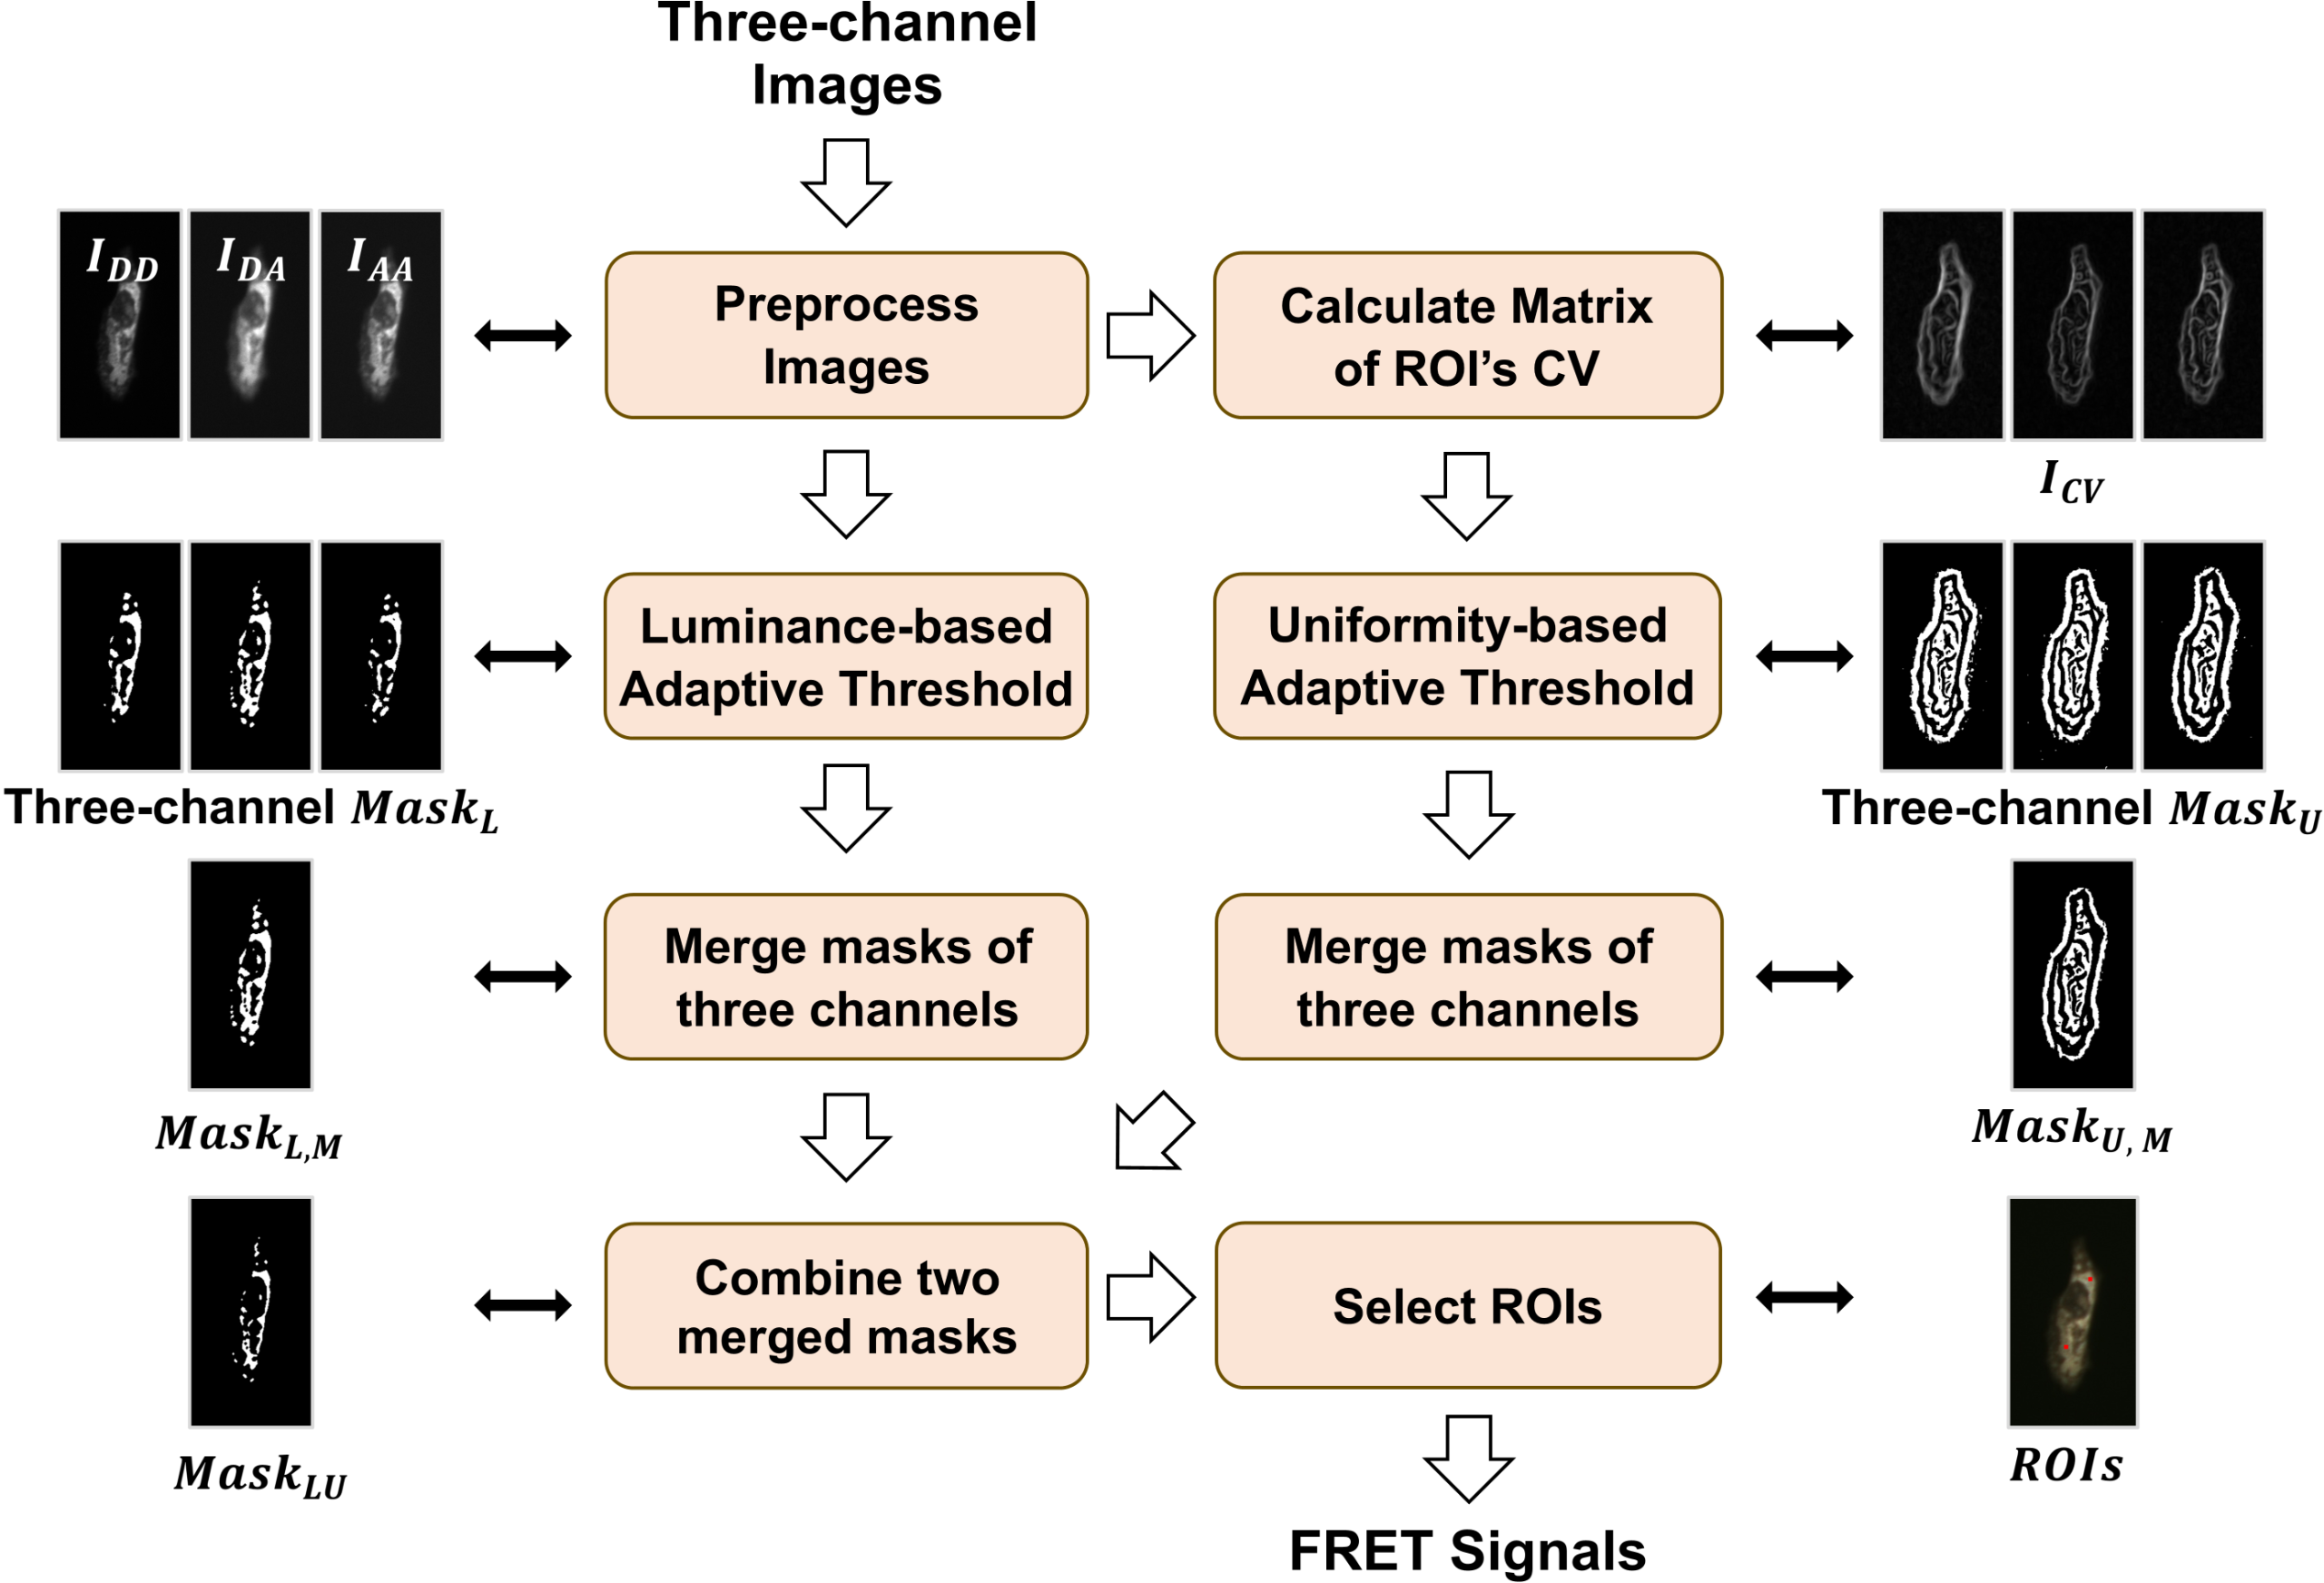
\includegraphics[width=1\linewidth]{../figures/4/LURS流程图.drawio.png}
\caption{LURS算法流程图}\label{fig1}
\end{figure*}

\subsection{基于LURS的自动FRET双杂交分析}
将LURS算法结合Fretha的数据计算处理能力,实现了全自动的FRET双杂交分析。
点击FRET图像处理模块左下角的“自动圈点”按钮,软件将会调用LURS算法进行自动ROI圈点生成,并记录到右侧的数据区。
计算过程中,Fretha界面通过进度条显示计算进度,方便用户查看。
基于LURS的自动圈点功能被封装在子线程服务中,不会影响Fretha前台界面显示和操作。

自动ROI圈点模块的业务流程及架构如图 \ref{fig:fret_auto_roi_flow} 所示。
架构层内的流程流转以实线表示,不同架构层之间的流程流转以虚线表示。
在实现自动圈点功能的流程转移中,发生在架构不同层之间的转移占更多数,而层内的流程转移相对较少,分层架构设计使得每个层内实现较好的封装,因此在实现复杂业务功能时,只专注于层和层之间的数据和流程切换即可。
\begin{figure}[htbp]
    \centering
    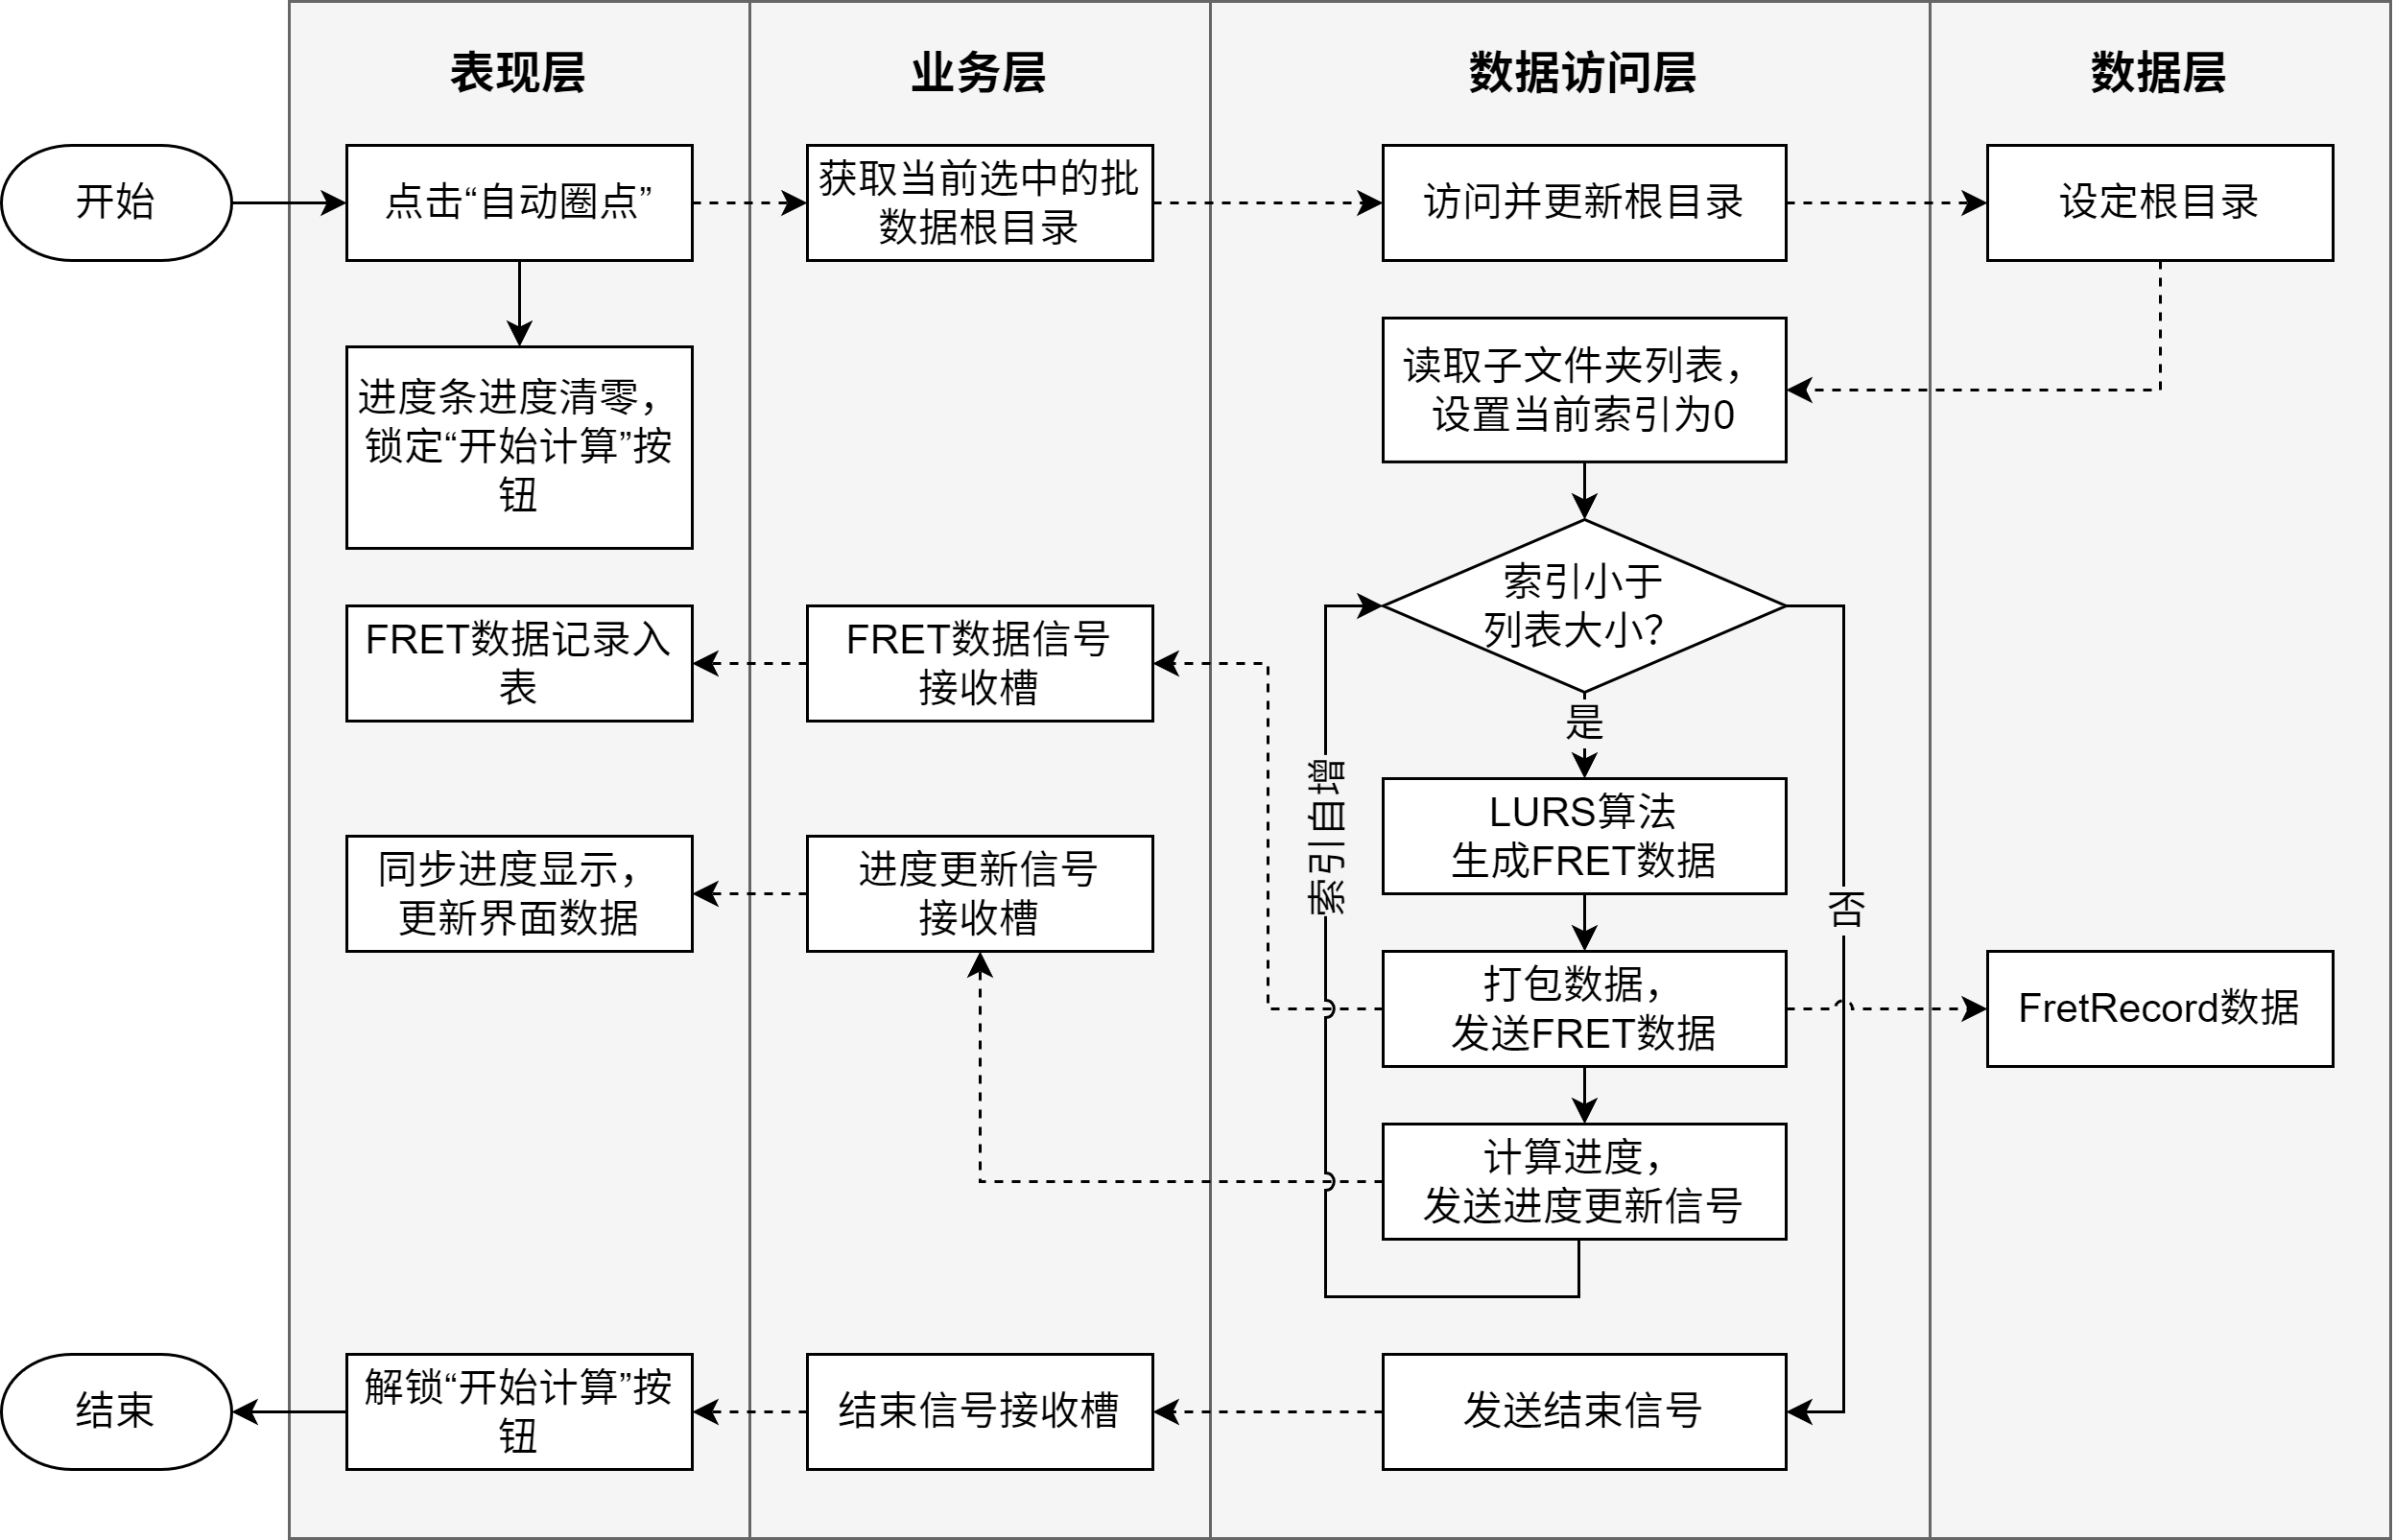
\includegraphics[width=1\linewidth]{../figures/4/自动ROI圈点在Fretha的流程.drawio.png}
    \caption{Fretha自动圈点功能流程}
    \label{fig:fret_auto_roi_flow}
\end{figure}

自动FRET双杂交分析方法采用DC-FRET方法,因为DC-FRET方法具有以下优势:
\begin{enumerate}
    \item 简化实验过程:与L-FRET方法相比,DC-FRET方法无需在中间分布状态下准备大量样本。相反,仅需准备相对较大$R_C$值和相对较小$R_C$值的样本,这减少了样本的制备和处理时间。
    \item 得出更稳定可靠的结果:DC-FRET中用于线性拟合的供体荧光能量转移效率$E_D$和受供体浓度比$R_C$数据是通过E-FRET和$3^3$-FRET方法进行定量测量的,该方法具有较高的准确性和稳定性,能够提供可靠的数据,使得线性拟合的结果更加稳定可靠。
\end{enumerate}

然而,DC-FRET方法在选择$R_C$或$1/R_C$的范围时需要一定经验。
如果所选范围过小,将会导致数据点不足,从而使结果的稳定性变差。
当拟合范围过大时,结果可能会不正确,因为所选数据不满足尽可能选择受体饱和结合或者供体饱和结合情况。
为了避免使用数据中的不稳定部分,本文中所有自动算法中进行的DC-FRET分析均遵循如下原则:
\begin{enumerate}
    \item 如果样本仅包含供体饱和的情况或仅包含受体饱和的情况,应选择$R_C$($1/R_C$)值相对较小的50\%的数据。
    \item 当受体饱和和供体饱和同时存在时,则应选择$R_C$($1/R_C$)值较小的25\%的数据。
\end{enumerate}

\section{实验结果}
\subsection{E-FRET和\texorpdfstring{$3^3$}{3^3}-FRET验证实验}
标准质粒验证实验的目的和质粒详情与第 \ref{sec:E-FRET和3^3-FRET处理结果} 节相同。
测量的结果列于表 \ref{tab:results_standard_plasmids} 中。
\begin{table*}[hbtp]
    \centering
    \caption{ 对标准质粒进行$3^3$-FRET和E-FRET测量的结果}
    \begin{tabularx}{\linewidth}{
    >{\centering\arraybackslash}p{1cm}
    >{\centering\arraybackslash}X
    >{\centering\arraybackslash}X
    >{\centering\arraybackslash}X
    >{\centering\arraybackslash}X
    >{\centering\arraybackslash}X
    >{\centering\arraybackslash}X}
    \toprule[1.5pt]
    \multirow{2}{*}{样本} & \multicolumn{3}{c}{测量结果} & \multicolumn{3}{c}{文献结果} \\
     & $E_{A}$ & $E_{D}$ & ${R_C}$ & $E_A$ & $E_{D}$ & $R_C$ \\
    \midrule
    C4Y  & $0.311\pm0.038$ & $0.293\pm0.023$ & $0.984\pm0.110$ & $0.296\pm0.001$ & $0.299\pm0.004$ & $1$ \\
    C10Y & $0.239\pm0.024$ & $0.214\pm0.022$ & $0.940\pm0.097$ & $0.228\pm0.002$ & $0.223\pm0.003$ & $1$ \\
    C40Y & $0.167\pm0.031$ & $0.152\pm0.014$ & $0.979\pm0.171$ & $0.156\pm0.002$ & $0.158\pm0.002$ & $1$ \\
    C80Y & $0.112\pm0.029$ & $0.114\pm0.020$ & $1.033\pm0.200$ & $0.116\pm0.001$ & $0.116\pm0.002$ & $1$ \\
    \bottomrule[1.5pt]
    \end{tabularx}
    \label{tab:results_standard_plasmids}
\end{table*}

通过对LURS提取的ROI的FRET信号进行计算和统计分析,结果表明:C4Y 的$E_A$值为 0.311,$E_D$值为 0.293,C10Y 的$E_A$值为 0.239,$E_D$值为 0.214,C40Y 的$E_A$值为 0.167,$E_D$值为 0.152,C80Y 的$E_A$值为 0.112,$E_D$值为 0.114。
与此同时,C4Y、C10Y、C40Y 和 C80Y 的$R_C$值分别为 0.984、0.940、0.979 和 1.033,与标准值1接近。
$E_A$、$E_D$和$R_C$的平均相对误差分别为 5.1\%、2.9\% 和 3.3\%。
所有质粒的$E_A$、$E_D$和$R_C$值都与已报道的值接近,这表明 LURS 算法能够成功提取出正确且有效的ROI,为FRET双杂交分析提供了从供体和受体角度的准确FRET效率等数据。

\subsection{FRET双杂交验证实验}
本节的测量方法和质粒详情与第 \ref{sec:模型质粒FRET双杂交验证实验} 节相同。
图 \ref{fig:results_model_plasmids} 展示了共表达 C32V / CVC 且含有游离的 C(C32V + C,CVC + C)(上半部分)或游离的 V(C32V + V,CVC + V)(下半部分)的活 MCF7 细胞的三张荧光图像(DD、AA 和 DA)(左侧),使用Fretha手动标注的ROI(中间),以及DC-FRET和L-FRET的结果图(右侧)。
\begin{figure}[htbp]
    \centering
    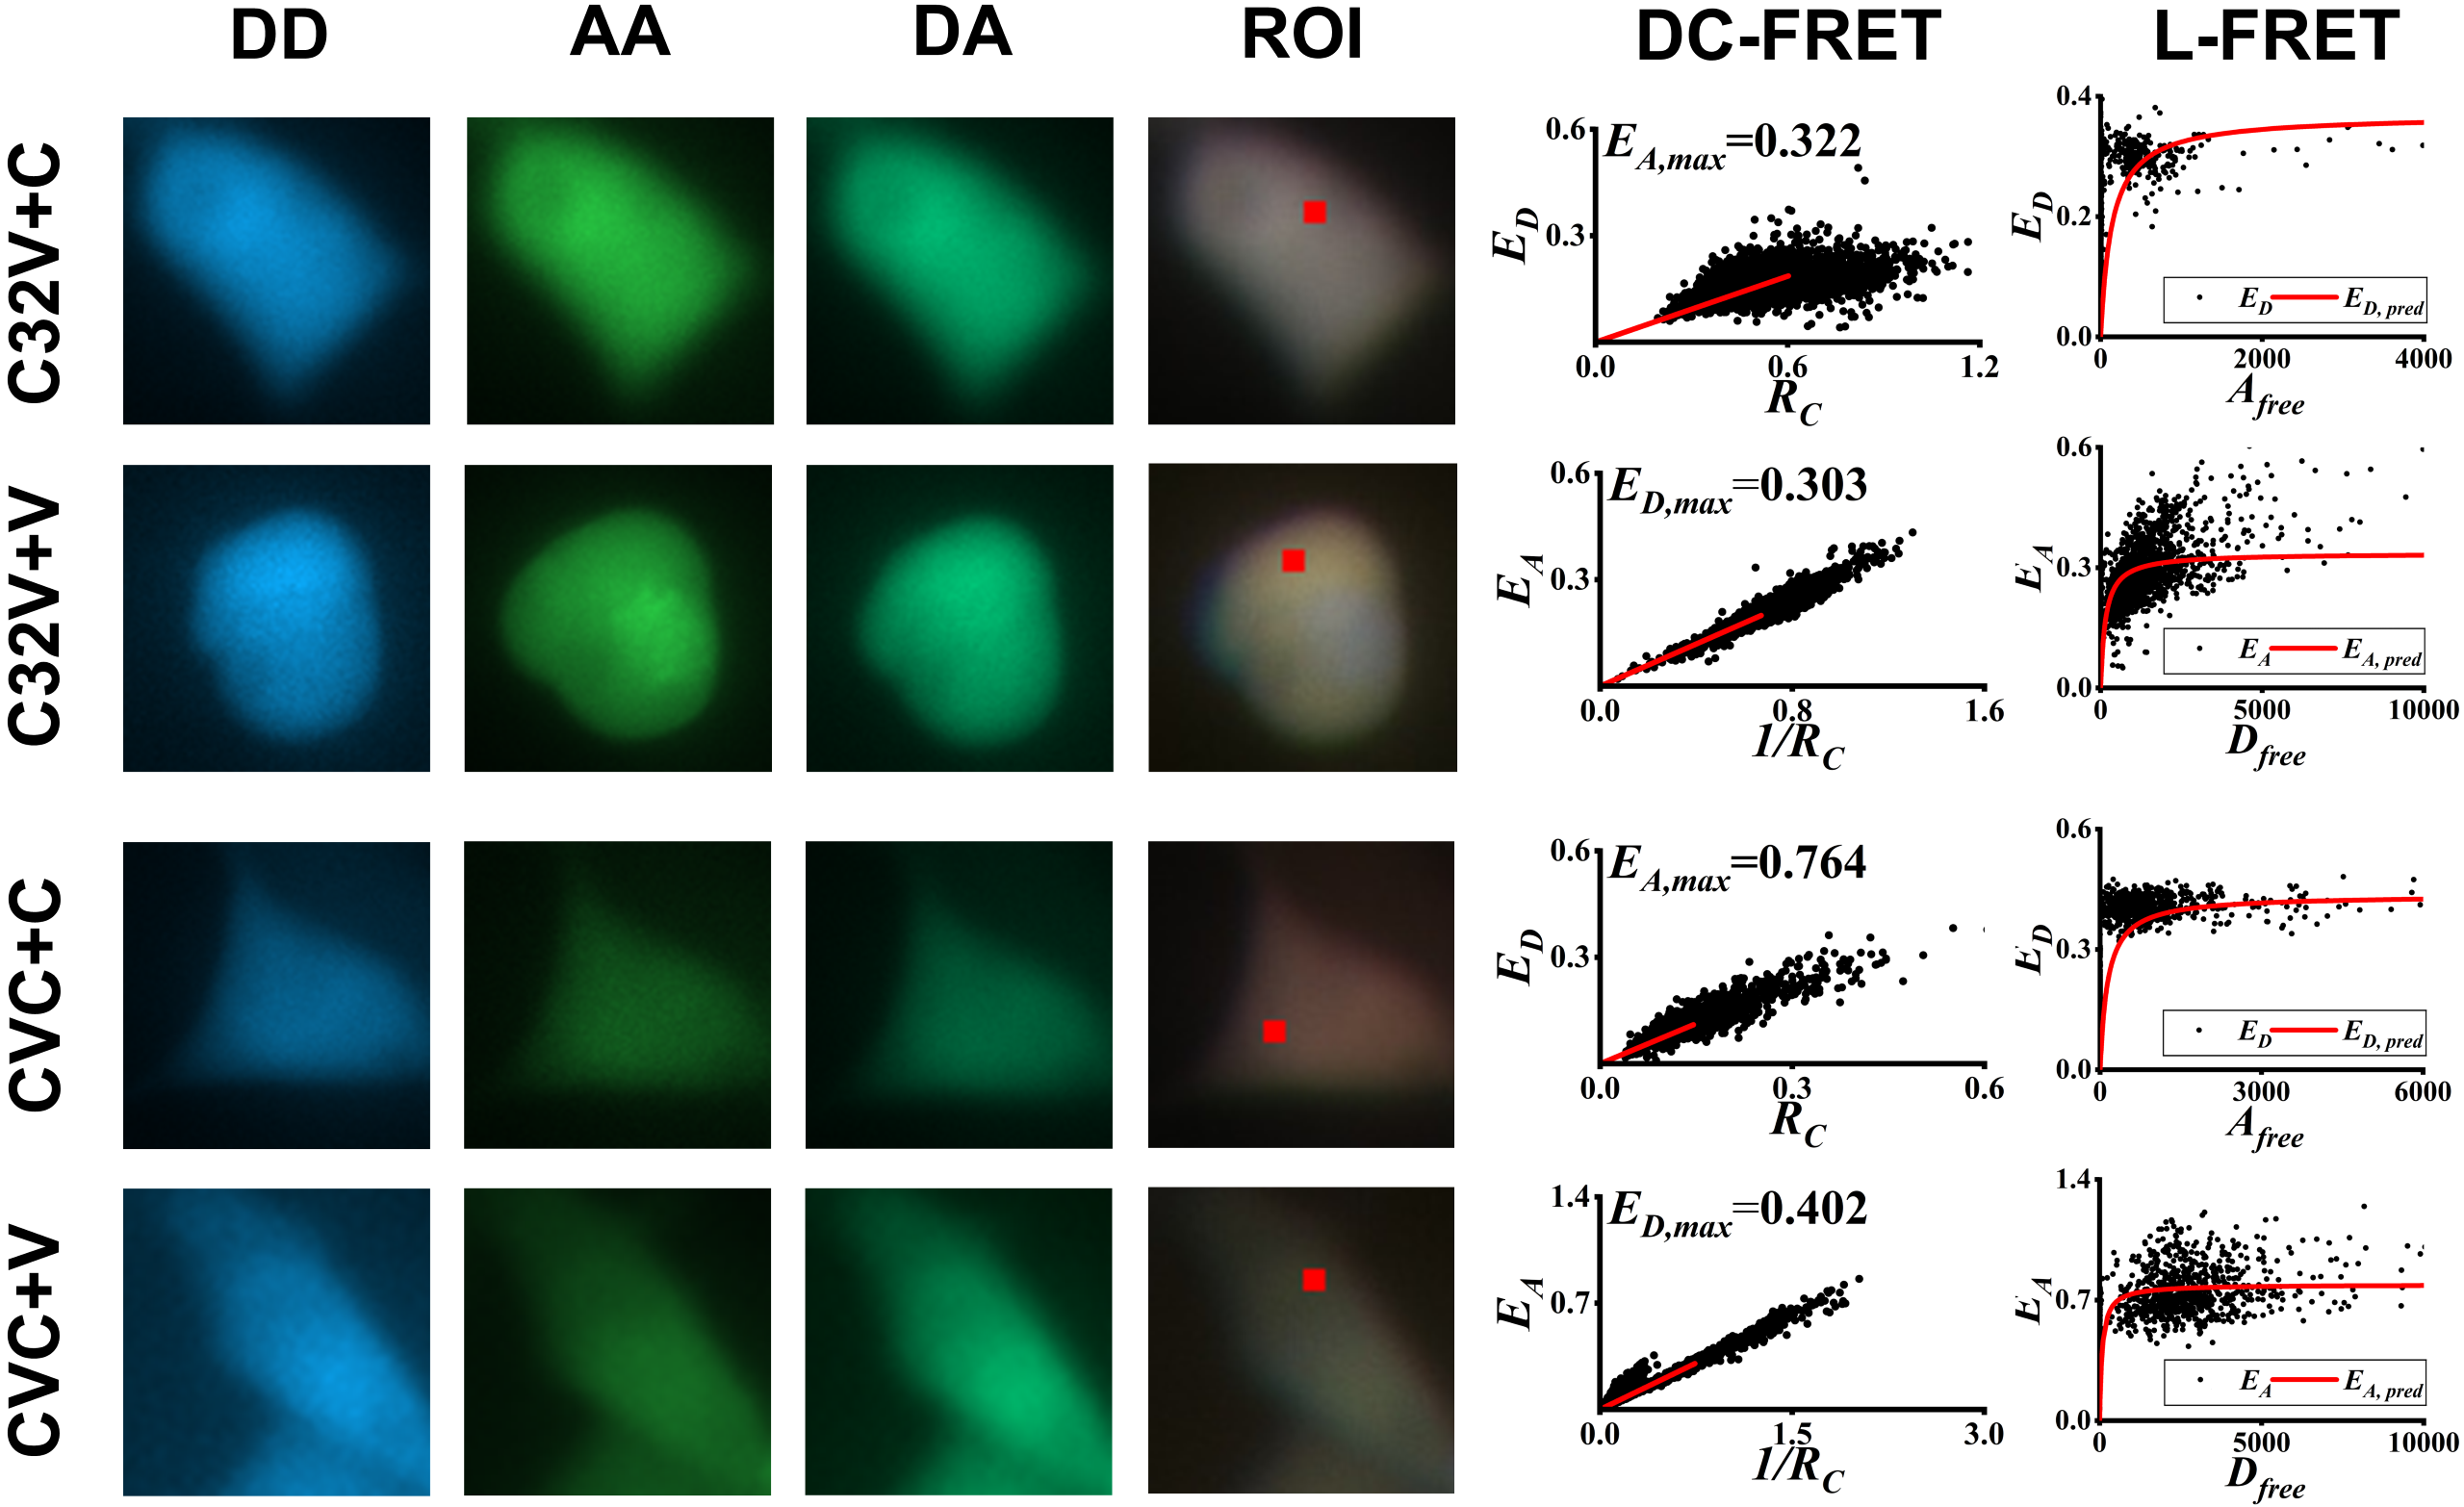
\includegraphics[width=1\linewidth]{../figures/4/LURS结果-模型质粒.drawio.png}
    \caption[模型质粒验证实验结果]{在存在游离供体或受体的情况下,分别通过DC-FRET和L-FRET方法对MCF7活细胞中标准质粒(C32V和CVC)的$E_{A, max}$、$E_{D, max}$和$n_D/n_A$进行自动FRET双杂交分析测量结果。}
    \label{fig:results_model_plasmids}
\end{figure}

C32V 和 CVC 质粒中Cerulean与Venus之间的结合化学计量比的实验测量结果见表 \ref{tab:results_model_plasmids}。
LURS结合DC-FRET,测量得到 C32V 质粒中的$E_{A,max}$为 0.322,$E_{D,max}$为 0.303,化学计量比($n_D/n_A$)为 1.063。
这个数值与 C32V 预期的供受体比例1:1非常接近。
对于 CVC 质粒,$E_{A,max}$、$E_{D,max}$和$n_D/n_A$的值分别为 0.764、0.402 和 1.900,所获得的结果与先前文献中报道的结果一致\upcite{koushik2006cerulean}。
结合L-FRET,LURS自动处理计算得到的 C32V 质粒中的$E_{D,max}$为 0.342,$E_{D,max}$为 0.372,化学计量比($n_D/n_A$)为 0.919。
对于 CVC 质粒,$E_{D,max}$、$E_{D,max}$和$n_D/n_A$的值分别为 0.791、0.442 和 1.790,与文献报道的结果一致\upcite{thaler2005quantitative}。
这些结果表明,LURS结合DC-FRET和L-FRET方法成功识别到了它们的化学计量比的差别,且计算出的化学计量比和文献结果的相对误差不超过 6\%,进一步证明了LURS算法提取高质量ROI的准确性。

\begin{table*}[htbp]
    \centering
    \caption{模型质粒的FRET双杂交分析结果}
    \begin{tabularx}{\linewidth}{
      >{\centering\arraybackslash}X
      >{\centering\arraybackslash}p{2.2cm}
      >{\centering\arraybackslash}p{2.2cm}
      >{\centering\arraybackslash}p{2.2cm}
      >{\centering\arraybackslash}X
      >{\centering\arraybackslash}X
      >{\centering\arraybackslash}X
      >{\centering\arraybackslash}X
      >{\centering\arraybackslash}X}
      \toprule[1.5pt]
      \multirow{2}{*}{样本} & \multicolumn{3}{c}{DC-FRET结果} & \multicolumn{3}{c}{L-FRET 结果} & \multicolumn{2}{c}{文献结果} \\
       & $E_{A,max}$ & $E_{D,max}$ & ${n_D/n_A}$ & $E_{D,max}$ & $E_{D,max}$ & ${n_D/n_A}$ & $E_{D,max}$ & $n_D/n_A$\\
      \midrule
      C32V & $0.322\pm0.041$ & $0.303\pm0.012$ & $1.063\pm0.143$ & $0.342$ & $0.372$ & $0.919$ & 0.311 & 1\\
      CVC  & $0.764\pm0.018$ & $0.402\pm0.024$ & $1.900\pm0.113$ & $0.791$ & $0.442$ & $1.790$ & 0.414 & 2\\
      \bottomrule[1.5pt]
      \hline %
      \end{tabularx}
    \label{tab:results_model_plasmids}
\end{table*}

\subsection{活细胞中 Bcl-xL-Bak 化学计量比的自动分析}
为了评估基于LURS算法的自动FRET双杂交分析的应用潜力,本节应用自动方法研究选择性 Bcl-xL 抑制剂 A1331852 存在下的 Bcl-xL-Bak 相互作用的化学计量比变化。
A1331852是具有口服活性的Bcl-xL的抑制剂,能够竞争性结合Bcl-xL,抑制Bcl-xL与促凋亡蛋白结合,从而抑制Bcl-xL的抗凋亡能力\upcite{wang2020discovery,kuusanmaki2023erythroid}。

为了对比LURS和深度学习方法的自动ROI选取效果,本节分别测试了对相同数据应用基于ilastik的方法基于SAM-Med2D的方法自动处理相同的输入数据,然后对比了不同方法的精确度和对药物敏感度的测试。
FRET定量计算、FRET双杂交计算均通过Fretha内部的相同算法进行处理。
在图像处理和ROI上,基于ilastik的方法通过少量标注交互,对输入的10个视野30张荧光细胞图像的像素分类为好细胞、坏细胞和背景区域,然后应用训练后的ilastik的模型进行自动分割,完成了对ROI的选取。
基于SAM-Med2D的方法通过对图像进行专家标注分为好细胞和背景区域,然后作为大模型输入的提示词(prompt)进行模型调整,最后输入实验用的数据完成自动分割。
在FRET双杂交分析方法上,由于DC-FRET的稳定性优于L-FRET,本节选用DC-FRET作为分析方法。

首先,如图 \ref {fig3} 所示,所有方法均能高精度测量 FRET 效率及化学计量比,并有效检测药物处理后的$E_{A,max}$、$E_{A,max}$和$n_D/n_A$值的下降。
这些结果表明,A1331852可破坏 Bcl-xL/Bak 相互作用,导致 受体中心的FRET 效率、供体中心的FRET效率和化学计量比均显著降低,且与手动分析结果趋势一致,验证了不同方法的测量一致性。
\begin{figure*}[!htb]
  \centering
  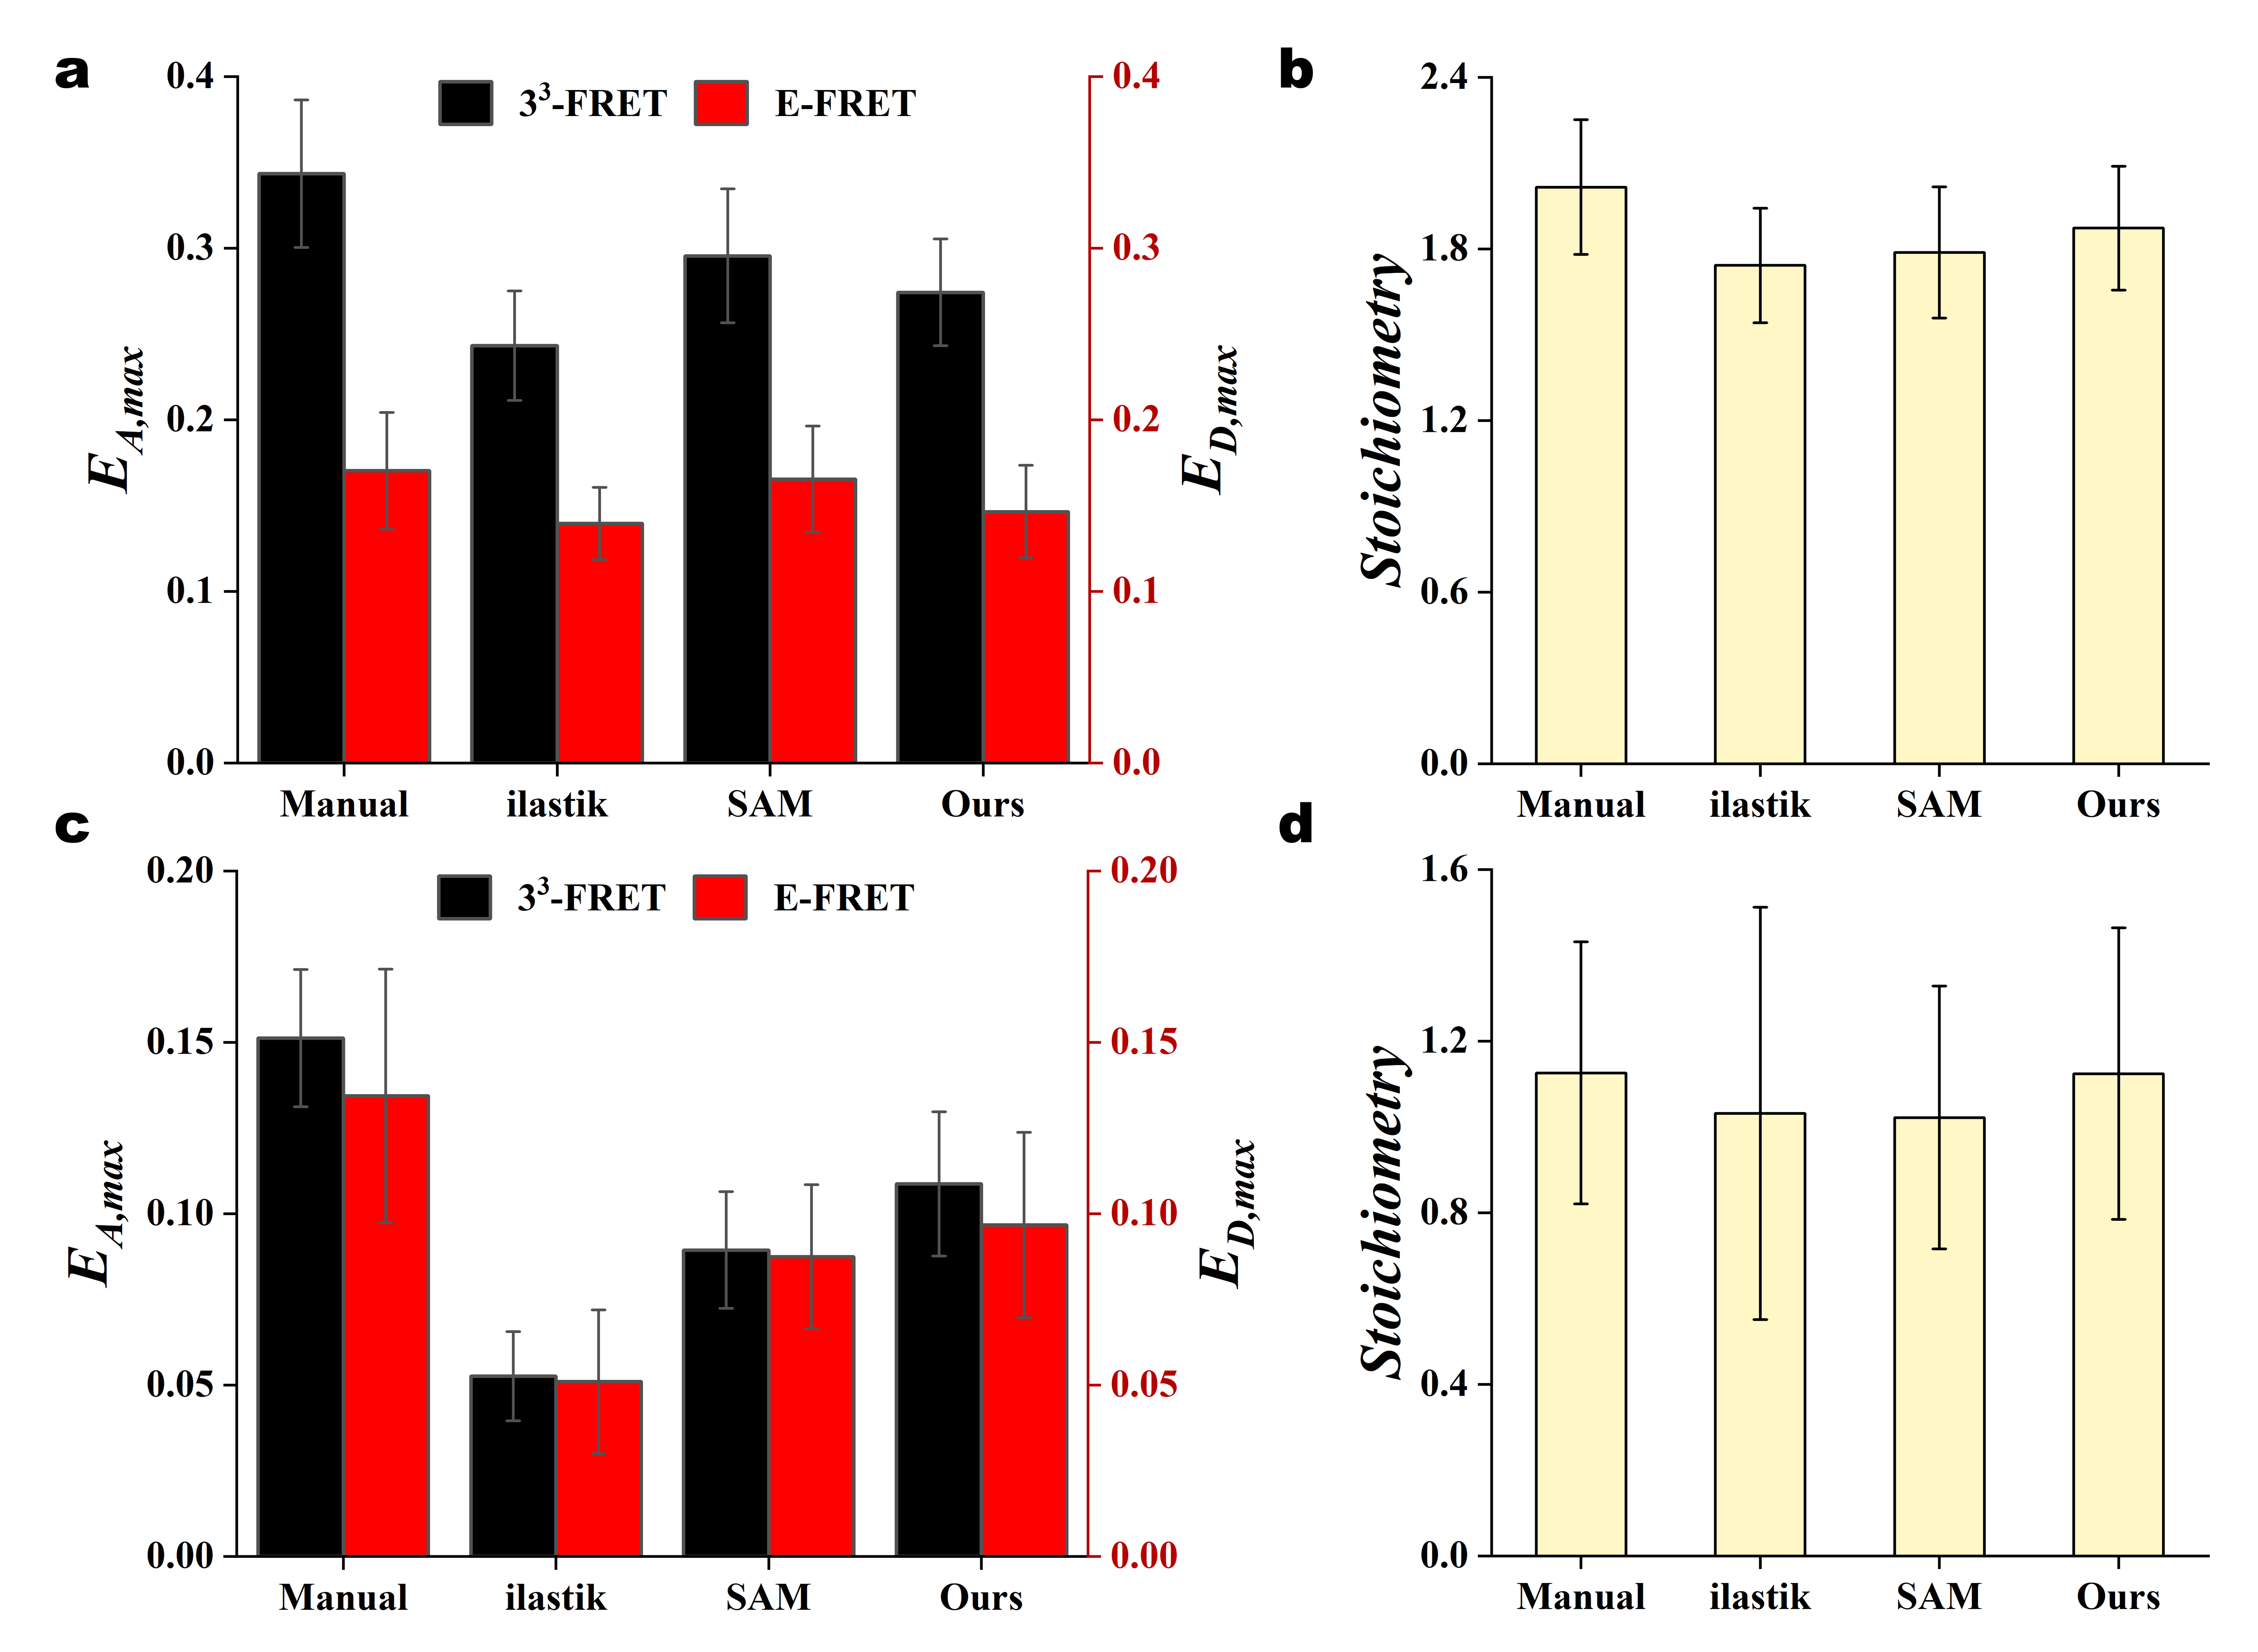
\includegraphics[width=1\linewidth]{../figures/4/4_方法对比.png}
  \caption[活细胞中 Bcl-xL-Bak 化学计量比的自动分析方法对比]{活细胞中 Bcl-xL-Bak 化学计量比的自动分析方法对比。手动、ilastik、SAM-Med2D及本方法计算的,A1331852处理前(a,b)和处理后(c,d)Bcl-xL-CFP与Bak-YFP结合的最大$3^3$-FRET(黑色)和E-FRET(红色)效率以及化学计量比(黄色)。}\label{fig3}
\end{figure*}

其次,本方法在$E_{A,max}$、$E_{D,max}$和$n_D/n_A$等参数的测量中表现出相较于SAM-Med2D和ilastik更高的整体准确性(见表 \ref{tab:comparison})。
在对照组中,本方法测得的$E_{A,max}$为$0.27\pm0.03$,$E_{D,max}$为$0.15\pm0.03$。
尽管SAM-Med2D测得的$E_{A,max}$($0.29\pm0.04$)更接近手动测量结果($0.34\pm0.04$),但本方法在$E_{D,max}$($0.15\pm0.03$,手动测量结果为$0.17\pm0.03$)和$n_D/n_A$($1.87\pm0.22$)上的偏差最小(手动测量结果为$2.01\pm0.14$),而SAM-Med2D($1.79\pm0.33$)和ilastik($1.74\pm0.19$)的化学计量比偏离更为显著。

在A1331852处理组中,本方法测得的所有参数均最接近手动测量结果,其中$E_{A,max}$为$0.11\pm0.02$,$E_{D,max}$为$0.10\pm0.03$(手动测量结果分别为$0.15\pm0.02$和$0.13\pm0.04$),显著优于SAM-Med2D($E_{A,max}$为$0.09\pm0.02$,$E_{D,max}$为$0.09\pm0.02$)和ilastik($E_{A,max}$为$0.05\pm0.01$,$E_{D,max}$为$0.05\pm0.02$)。
特别值得注意的是,本方法测得的化学计量比$n_D/n_A$($1.12\pm0.33$)与手动测量结果($1.12\pm0.30$)完全一致,而SAM-Med2D($1.02\pm0.30$)和ilastik($1.03\pm0.48$)的结果则表现出更大的离散性。
这些结果充分表明,本方法对FRET效率和化学计量比的定量分析具有更高的稳健性。
\begin{table*}[htbp]
  \centering
  \caption[活细胞中 Bcl-xL-Bak 化学计量比的自动分析方法对比]{手动、基于ilastik、基于SAM-Med2D 及Fretha自动方法测量 A1331852 处理前后 Bcl-xL-CFP 与 Bak-YFP 结合的 DC-FRET 双杂交分析结果。}
  \begin{tabularx}{\linewidth}{
  >{\centering\arraybackslash}p{2.2cm}
  >{\centering\arraybackslash}X
  >{\centering\arraybackslash}X
  >{\centering\arraybackslash}X
  >{\centering\arraybackslash}X
  >{\centering\arraybackslash}X
  >{\centering\arraybackslash}X}
  \toprule[1.5pt]
  \multirow{2}{*}{方法} & \multicolumn{3}{c}{对照组} & \multicolumn{3}{c}{加药组}  \\
   & $E_{A,max}$ & $E_{D,max}$ & ${n_D/n_A}$ & $E_{A,max}$ & $E_{D,max}$ & ${n_D/n_A}$ \\
  \midrule
  Manual    & $0.34\pm0.04$ & $0.17\pm0.03$ & $2.01\pm0.14$ & $0.15\pm0.02$ & $0.13\pm0.04$ & $1.12\pm0.30$ \\
  ilastik   & $0.24\pm0.03$ & $0.14\pm0.02$ & $1.74\pm0.19$ & $0.05\pm0.01$ & $0.05\pm0.02$ & $1.03\pm0.48$ \\
  SAM-Med2D & $0.29\pm0.04$ & $0.17\pm0.05$ & $1.79\pm0.33$ & $0.09\pm0.02$ & $0.09\pm0.02$ & $1.02\pm0.30$ \\
  Ours      & $0.27\pm0.03$ & $0.15\pm0.03$ & $1.87\pm0.22$ & $0.11\pm0.02$ & $0.10\pm0.03$ & $1.12\pm0.33$ \\
  \bottomrule[1.5pt]
  \hline %
  \end{tabularx}
  \label{tab:comparison}
\end{table*}

\subsection{自动分析算法性能对比}
在相同硬件配置(Intel\textsuperscript{\textregistered} Xeon E5-2678 v3 @ 2.50GHz处理器,NVIDIA\textsuperscript{\textregistered} GeForce RTX 3090 GPU)下,我们对LURS算法与两种基于深度学习的自动ROI提取方法(ilastik和SAM-Med2D)进行了系统性性能对比。

基于LURS和Fretha的自动FRET双杂交分析流程通过改进四个方面改进将时间花费从传统手动处理的3.5 - 7小时缩短至30分钟,节省了85.7\%以上的时间:
\begin{enumerate}
  \item 实时LURS驱动的感兴趣区域分割消除了每个样本2.5至3小时的手动区域选择和背景校正时间;
  \item 简化的FRET/DC-FRET计算模块将计算和拟合时间从1小时缩短至不足5分钟;
  \item 与数据处理平台直接集成的自动化数据格式转换流程消除了1小时的手动数据转换步骤;
  \item Fretha平台支持的数据筛选和质量控制,以及易于数据在处理的特效,将数据检查和再处理时间从1小时减少至20分钟。
\end{enumerate}

如表 \ref{tab:性能对比} 所示,LURS方法在1.4GB数据集(包含30个视野的药物处理组和对照组)中仅需10秒即可提取1515个可用的ROI,单ROI处理时间低至6.6 ms。
相比之下,ilastik和SAM-Med2D的单ROI处理时间分别为35.2 ms和50.7 ms,LURS的速度较ilastik提升5.3倍,较SAM-Med2D提升7.7倍。
\begin{table*}[htbp]
  \centering
  \caption{不同算法的性能对比}
  \begin{tabular}{cccc}
  \toprule[1.5pt]
  方法 & 单ROI处理时间(ms) & 内存占用 & 硬件要求 \\
  \midrule
  LURS & 6.6 & 约800 MB & CPU \\
  ilastik & 35.2 & 约1.8 GB & GPU/CPU \\
  SAM-Med2D & 50.7 & 约14 GB & GPU \\
  \bottomrule[1.5pt]
  \end{tabular}
  \label{tab:性能对比}
\end{table*}

内存利用率方面,LURS运行时仅占用约800 MB内存,分别为ilastik(约1.8 GB)的43.4\%和SAM-Med2D(约14 GB)的5.6\%。
这意味着在普通内存容量的计算机上,LURS和Fretha即可进行自动化图像处理和FRET双杂交分析。
此外,LURS完全依赖CPU资源,无需专用GPU加速或其他额外硬件投入即可方便集成到实时显微镜成像系统中。  

\section{本章小结}
本章提出了一种基于亮度均匀性的自动 ROI 选择算法 (LURS),以解决传统 FRET 双杂交分析技术中ROI标注依赖人工的问题,实现了自动的FRET双杂交分析。
LURS算法通过高斯平滑预处理,既实现了对噪声的抑制,又保留了荧光信号的强度信息。
通过局部明度和变异系数双重指标的自适应阈值分割,LURS保留了细胞中明度较高且荧光突变小的区域,从而选取了高质量的ROI。
结合LURS算法和DC-FRET方法的自动数据选择,本章成功实现了整个 FRET 双杂交分析过程的自动化,并将其作为一个自动数据处理的功能集成到了Fretha中,丰富了软件的功能。
应用基于LURS的自动FRET双杂交分析方法,在标准质粒 C4Y/C10Y/C40Y/C80Y 的 $3^3$-FRET和E-FRET 验证实验中,$E_A$、$E_D$和$R_C$测量值相对文献值的平均相对误差分别为 5.1\% 和 2.9\%和3.3\%。
在FRET双杂交分析验证实验中模型质粒 C32V 和 CVC 的化学计量比分析中,测量的 $n_D/n_A$ 值分别为 $1.063 \pm 0.143$ 和 $1.900 \pm 0.113$,与理论值 1:1 和 2:1 高度吻合,且计算效率较人工处理提升 85.7\% 以上。
应用自动算法分析A1331852药物处理的活细胞中Bcl-xL-Bak之间的相互作用,LURS结合DC-FRET算法敏锐地检测到Bcl-xL和Bak之间的作用计量从$1.87 \pm 0.22$下降到$1.12 \pm 0.33$,在ilastik、SAM-Med2D等方法中最接近人工手动处理的标准结果。
实验结果表明,基于LURS算法的自动FRET双杂交分析方法具有准确性高、速度快、成本低等优点,为高通量FRET双杂交分析检测和药物筛选等研究提供了技术支撑。